\documentclass{article}

% if you need to pass options to natbib, use, e.g.:
% \PassOptionsToPackage{numbers, compress}{natbib}
% before loading nips_2016
%
% to avoid loading the natbib package, add option nonatbib:
% \usepackage[nonatbib]{nips_2016}

\usepackage[final]{nips_2016}

% to compile a camera-ready version, add the [final] option, e.g.:
% \usepackage[final]{nips_2016}

\usepackage[utf8]{inputenc} % allow utf-8 input
\usepackage[T1]{fontenc}    % use 8-bit T1 fonts
\usepackage{hyperref}       % hyperlinks
\usepackage{url}            % simple URL typesetting
\usepackage{booktabs}       % professional-quality tables
\usepackage{amsfonts}       % blackboard math symbols
\usepackage{nicefrac}       % compact symbols for 1/2, etc.
\usepackage{microtype}      % microtypography
\usepackage{xcolor, graphicx, subcaption, float}

\newcommand{\selfnote}[1]{\footnote{\textcolor{red}{#1}}}
\newcommand{\domainDoubt}[1]{\footnote{\textcolor{teal}{#1}}}
\newcommand{\technicalDoubt}[1]{\footnote{\textcolor{blue}{#1}}}

\title{Commuter classification and behavior clustering: Beijing use case}

% The \author macro works with any number of authors. There are two
% commands used to separate the names and addresses of multiple
% authors: \And and \AND.
%
% Using \And between authors leaves it to LaTeX to determine where to
% break the lines. Using \AND forces a line break at that point. So,
% if LaTeX puts 3 of 4 authors names on the first line, and the last
% on the second line, try using \AND instead of \And before the third
% author name.

\author{
  Selene Baez  Santamaria \\
  \texttt{s.baezsantamaria@student.vu.nl}
}

\begin{document}
% \nipsfinalcopy is no longer used

\maketitle

\begin{abstract}
  Public transportation, centered on subway and bus networks, is an data-rich domain that can benefit from data mining and machine learning techniques. The classification of commuters versus non-commuters/occasional travelers can help government, transport management and operators to better target their policies in order to improve the transportation network in large cities. Furthermore, characterizing commuters by behavior clustering can bring deeper insight into their needs and routines as a whole. 
  This project proposes the usage of ensemble models for classification and clustering of public transport users. For this purpose, transit card data will be used, available from the city of Beijing, China. 
\end{abstract}

\newpage

\tableofcontents

\newpage
\section{Introduction}

\subsection{Transportation domain}
Urban public transportation includes systems that are available for use by anyone in urban areas. Its facilities are commonly composed by buses, subway/metro lines, light rails, tramways, trains and others. As a network, they provide service for the majority of citizens in urban areas. \citep{vuchic1900urban}

Figure \ref{fig:transportation/passenger} shows the passsenger transport usage, as million passengers per kilometer. This represents the transport of a passenger for one kilometer. From the top image note that United Stated, China, Germany, France, Italy, and United Kingdom contitute the six countries with the most passenger transport, according to their reported data from 2015 or later \cite{OECD2017passenger}. 

Furthermore, historical data in the bottom image reveals the 15 years behavior for each of the aforementioned countries. Most of the countries show stability, with increase or decrease of less than .10 million passengers for European countries, and .5 million passengers for United States. China, however, shows a trend with steep increase for most of the selected years. In fact, comparing its less than 1.2 million passengers in 2000, China doubled its public transport usage to 2.4 million passengers in 2015. 

\begin{figure}[H]
  \centering
  \begin{subfigure}[b]{.8\textwidth}
  	\centering
  	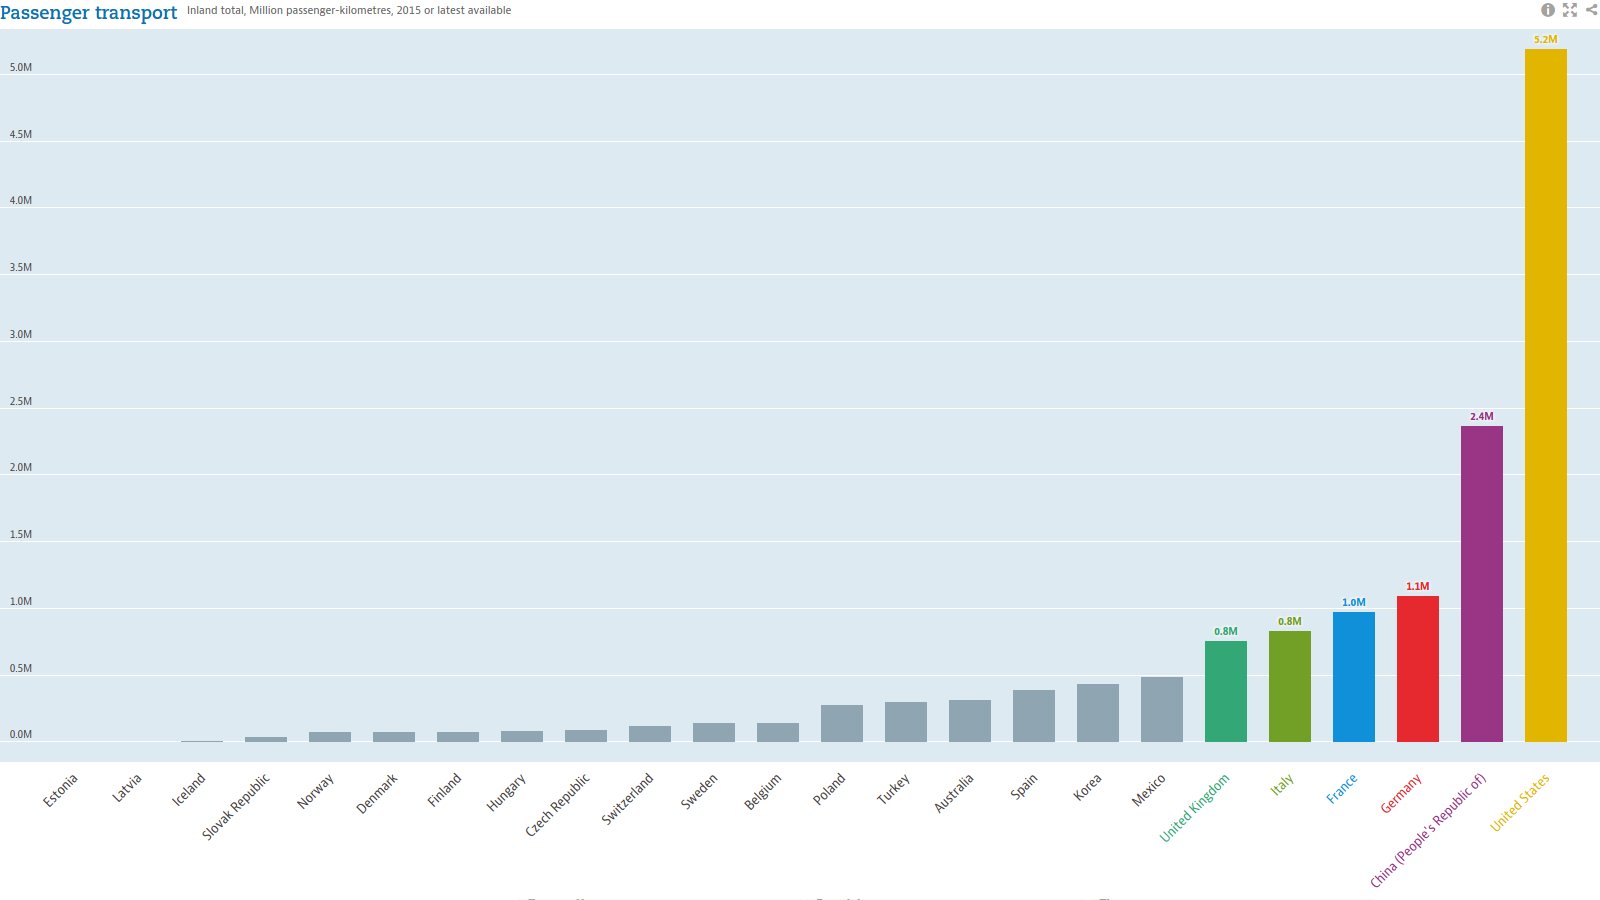
\includegraphics[width=\linewidth]{./images/OECD_passengers_absolute.png}
  	\caption{Passenger transport data, per country.}
  \end{subfigure}
  \begin{subfigure}[b]{.8\textwidth}
  	\centering
  	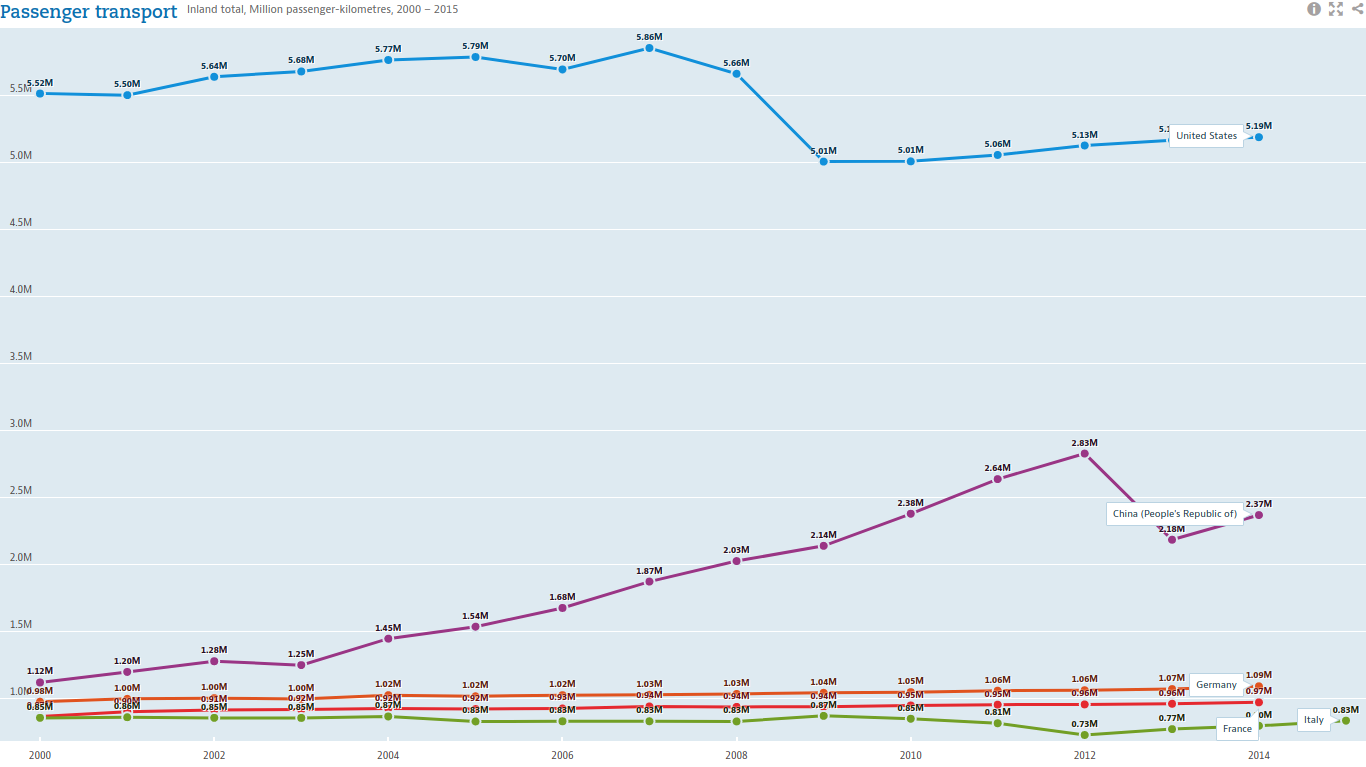
\includegraphics[width=\linewidth]{./images/OECD_passengers_increase.png}
  	\caption{Historical data for the top six countries with most passenger transport usage.}
  \end{subfigure}
  \caption{OECD countries and their passenger transportation data.}
  	\label{fig:transportation/passenger}
\end{figure}

The usage of the public transport network as a whole has a significant environmental impact, affecting noise and air pollution. \selfnote{references}. 


Public transportation also relates to energetic demand, since its facilities are mostly petroleum or electrical based. In terms of global energy consumption, passenger transportation accounts for about 25\% of the total world energy consumption. Furthermore, the tarnsportation sector consupmtion increases at an annual average rate of 1.4\% \cite{eia2016energy}. This may bring further economical implications.

In the last years, smart cards systems appeared, making it possible to track travelers and facilitating the fare collection. Examples are Octopus card in Hong Kong, Oyster card in London, OV-chipcard in The Netherlands and IC card in Beijing, to name a few.


\subsubsection{Who are the commuters?}
A major proportion of public transport users is represented by commuters. These are regular users of public transit, with regularity in the boarding times/stops. 

Driven by a routine, commuters travel back and forth from specific places, commonly represented by home to work/school trips. As commuters use public transit almost daily, or with a regular temporal pattern, the  conditions of the public network directly influence commuter's personal life and generally impacts their quality of life \selfnote{reference}. If the commuting experience is bad, daily travel can bring sorrow to users. Bad experiences may include excessively long commuting time, crowded spaces, inconvenient transfers, elevated prices, low-quality of facilities, and others. 

Identifying commuters can help in the long-term planning (sustainable) of public transportation. Policies for improving the overall experience and aid urban areas on a large scale.

Transportation follows swarm behavior. Based on individual travels and routines, on a larger scale travelers exhibit peculiar characteristics. Both levels of understanding are crucial.   

\subsection{The city of Beijing}
Beijing special case for urbanization. Number of people is massive \selfnote{reference}

Pollution in Beijing \selfnote{reference}

Beijing has more than 1000 bus routes and 18 subway lines, and it continues to expand every year. This results in more than 28,000 stops combined. \selfnote{reference Beijing transportation center}. 

Additionally, Beijing has implemented several Bike sharing systems, with specific dropping stations. \domainDoubt{where to get this info}.

Number of users per day.

By the usage of smart transit cards, collection of payment and transaction monitoring is possible. Buses, subways, bikes and taxis are monitored. Real time and historical data is available. Over 90\% of public transit users are smart card holders. \selfnote{reference}

\subsection{Motivation}
Interdisciplinary study between Artificial Intelligence and Metropolitan Transportation. Introduce data mining techniques to a data rich domain. 

Relevance of project on both areas. 

\subsubsection{Societal context}
Commuters use the public transport network regularly to go to work, school or other follow other routines. They need reliable means of transportation. \selfnote{reference: what do commuters care about}.

The city of Beijing faces a large imbalance between residential and working areas. \selfnote{reference}. Targeting this group brings the largest benefits to the public.  

Government, transport management and operators can gain spatial and temporal insight. This insight can lead to tangible results, policies and counter measures increasing efficiency of network, adjustable travel fares used as incentives to relieve peak hours, urban planning for residential and industrial land use, and others \selfnote{reference}

\subsubsection{Scientific context}
Usage of machine learning of data mining has been limited. Current broadly used method is surveys to reach travelers on individual level and aggregated measurements for gathering  their collective behavior. The analysis is usually done with statistical methodology. 

Surveys are costly and based on self-report, which by itself has bias problems. Other problems are small population and non-representative samples. 

Aggregated methods miss the interactions between individuals that cause the collective behavior. 

Technology has reached the data collection point, but has yet to reach the analysis part. Transit cards are capable of recording spatio-temporal information at an individual level over long periods of time. This generates large amounts of data. 

Many prediction algorithms available. Constant refinement, state of the art must be applied to real life and large impact situations. Domain experts must focus on analyzing insights and using them, not on techniques for curating and making sense out of raw data. 

\subsection{Thesis organization}
This Thesis is organized as follows:

First we do a literature review for previous work on mining transit data and for specific state-of-the art methodologies. Consequently, we establish the scope and objectives of this project. We continue to describe the methodology thoroughly, including the data and the approach. Following this description, we identify three distinct stages of the project and report their corresponding experimentation. Then, we discuss the findings and gather conclusions. Finally, future work opportunities are explored. 


\newpage
\section{Literature review}

\subsection{Data mining on transit card data}
Preprocess data by Wang in BJUT lab. \cite{wang2014research}

Data mining to identify transit use cycles in Canadian smart card data \cite{morency2007measuring}

Density Based Scanning Algorithm with Noise to classify travelers according to their travel patterns.  \cite{ma2013mining}

Passenger segmentation by K-means clustering \cite{bhaskar2015passenger}

Machine learning for commuters identification. SVM with 94\% accuracy. \cite{tu2016impact}

11 distinct clusters of users with similar activity and demographic attributes \cite{langlois2016inferring}

The latest work on the field corresponds to Ma et Al \cite{ma2017understanding}. The objective of their work is to determine a scoring function for travelers that can correctly identify them as commuters, or non-commuters. In their work, they cluster stops using an improved DBSCAN algorithm. They engineer features for representing the frequency in which travelers follow spatio-temporal patterns. Travelers are then clustered according to these features following the ISODATA algorithm. As an output of the clustering, optimal cutoff levels in the scoring function were determined. As a result, evaluating a traveler does not depend on clustering centroids, but only on calculating the commuting score. This, as expressed by the authors, reduces computing time and treats each traveler independently from the others, which is not true for clustering algorithms.

A common practice, as used by \cite{ma2017understanding} and \cite{langlois2016inferring} is to divide the day into -hourly or half-and-hour- time bins.

\subsection{Classifying and clustering spatio-temporal data}
Ensemble methods

Classifiers in the transportation domain


\newpage
\section{Research objective}
Objective is to identify and characterize commuters in the city of Beijing by using IC card data. Find patterns in the spatio-temporal data of public transport travelers. 

\subsection{Research questions}
\begin{enumerate}
\item How accurately can commuters and non-commuters be identified using an ensemble model? How does this compare to the previous SVM model?
\item What is the minimal set of information needed from IC card data to reach an acceptable accuracy in classification?
\item To what extent is clustering commuters by its behavior informative to transportation specialists? 
\end{enumerate}

\subsubsection{Definition of terms}
A commuter is a public transit user whose IC card data reveals repeatable patterns in time and space over a working week (5 days, Monday through Friday).

A trip is a sequence of IC card transactions, including transfers, with an origin and destination. A trip is also represented as a record in the data, as it will be further explained in Section \ref{sec:data}

A transfer is a change in transportation mode. Transportation modes include Bus, Subway, and Bike. Transfers can then be: bus-bus, bus-subway, bus-bike, subway-bus, subway-bike, bike-bus, bike-subway or bike-bike. Changes between subway lines are not recorded. \domainDoubt{transfer possible?} 

We make the assumption that IC card IDs and users have a one to one relationship, meaning each user has exactly one card and each card is used by exactly one user. \domainDoubt{reasonable assumption?}

\subsection{Scope and structure}
\selfnote{revise this part}
The coverage of this Thesis is divided in three main stages: 

\begin{itemize}
\item[Part one]: classify commuters versus non-commuters. Ensemble model compared to SVM

\item[Part two]: the set of features will be revised to disregard redundant information. A second comparison with Tu\cite{tu2016impact}'s SVM model will be made. 

\item[Part three]: commuters will be further clustered according to patterns in their behaviors that will emerge from all variables of the IC card data. The clusters will be analyzed and interpreted to find distinctive characteristics that may be judged as useful by transportation specialists. 
\end{itemize}

\selfnote{better itemize bullets}


\newpage
\section{Methodology}
\subsection{The data}
\label{sec:data}
Every record int he data represents a trip performed by a specific IC card. As such, it contains the following data fields:

\begin{itemize}
\item Data date: Year, month and day that the trip was made
\item Card code: card identification number
\item Path link: Mode of transportation. B for bus, R for subway, Y for bicycle. Transfers between modes are shown by a dash. \footnote{Example: B-B is Bus to Bus.} \domainDoubt{calculated column? there are some inconsistencies between this and transfer detail}
\item Travel time: Time spent in vehicles, measured in milliseconds
\item Travel distance: Distance traveled, measured in meters \selfnote{as measured by route? or start-end stops}
\item Transfer number: Number of changes in travel mode during the trip. Regarding transfers between same travel mode, bus to bus, and bike to bike transfers are counted. Subway to subway transfers are ignored. 
\item Transfer average time: Time spent in transfer, divided by number of transfers. , Measured in milliseconds \selfnote{calculated column?}
\item Transfer total time: Total time spent in transfer, measured in milliseconds
\item Start/End time: Time stamp of when the trip started/ended. Date and time with milliseconds precision
%Traffic zones
\item On/Off small traffic area: Integer from 1 to 1911
\item On/Off middle traffic area: Integer from 1 to 389
\item On/Off big traffic area: Integer from 1 to 60
%Municipal zones
\item On/Off ring road: Integer 1 to 6
\item On/Off area: Integer from 1 to 18 corresponding to the district/county for boarding and alighting, correspondingly. See Figure \ref{fig:data/18areas} \selfnote{reference} \selfnote{include in preprocessing dictionary?} 
%http://www.ebeijing.gov.cn/Government/Administration_region/}
\item ID: record identification number created by joining the following: hour | time stamp of beginning of trip | card code
\item Transfer detail: Station name, line number, mode of transportation
\end{itemize}

The traffic zones (small, middle and big areas) are divided by the Planning and Designing Institute in Beijing\selfnote{reference}. They are specific in different degrees. In general, the division principles correspond to the geopolitical environment and administrative planning, for example roads, villages and others. The 6 ring road and 18 areas are divided by the Beijing Municipal Government \selfnote{reference}. The division is unique in Beijing. According to domain expert Liang Quan, these divisions are sufficiently informative for traffic analysis. \technicalDoubt{how to quote a person}

\begin{figure}
  \centering
  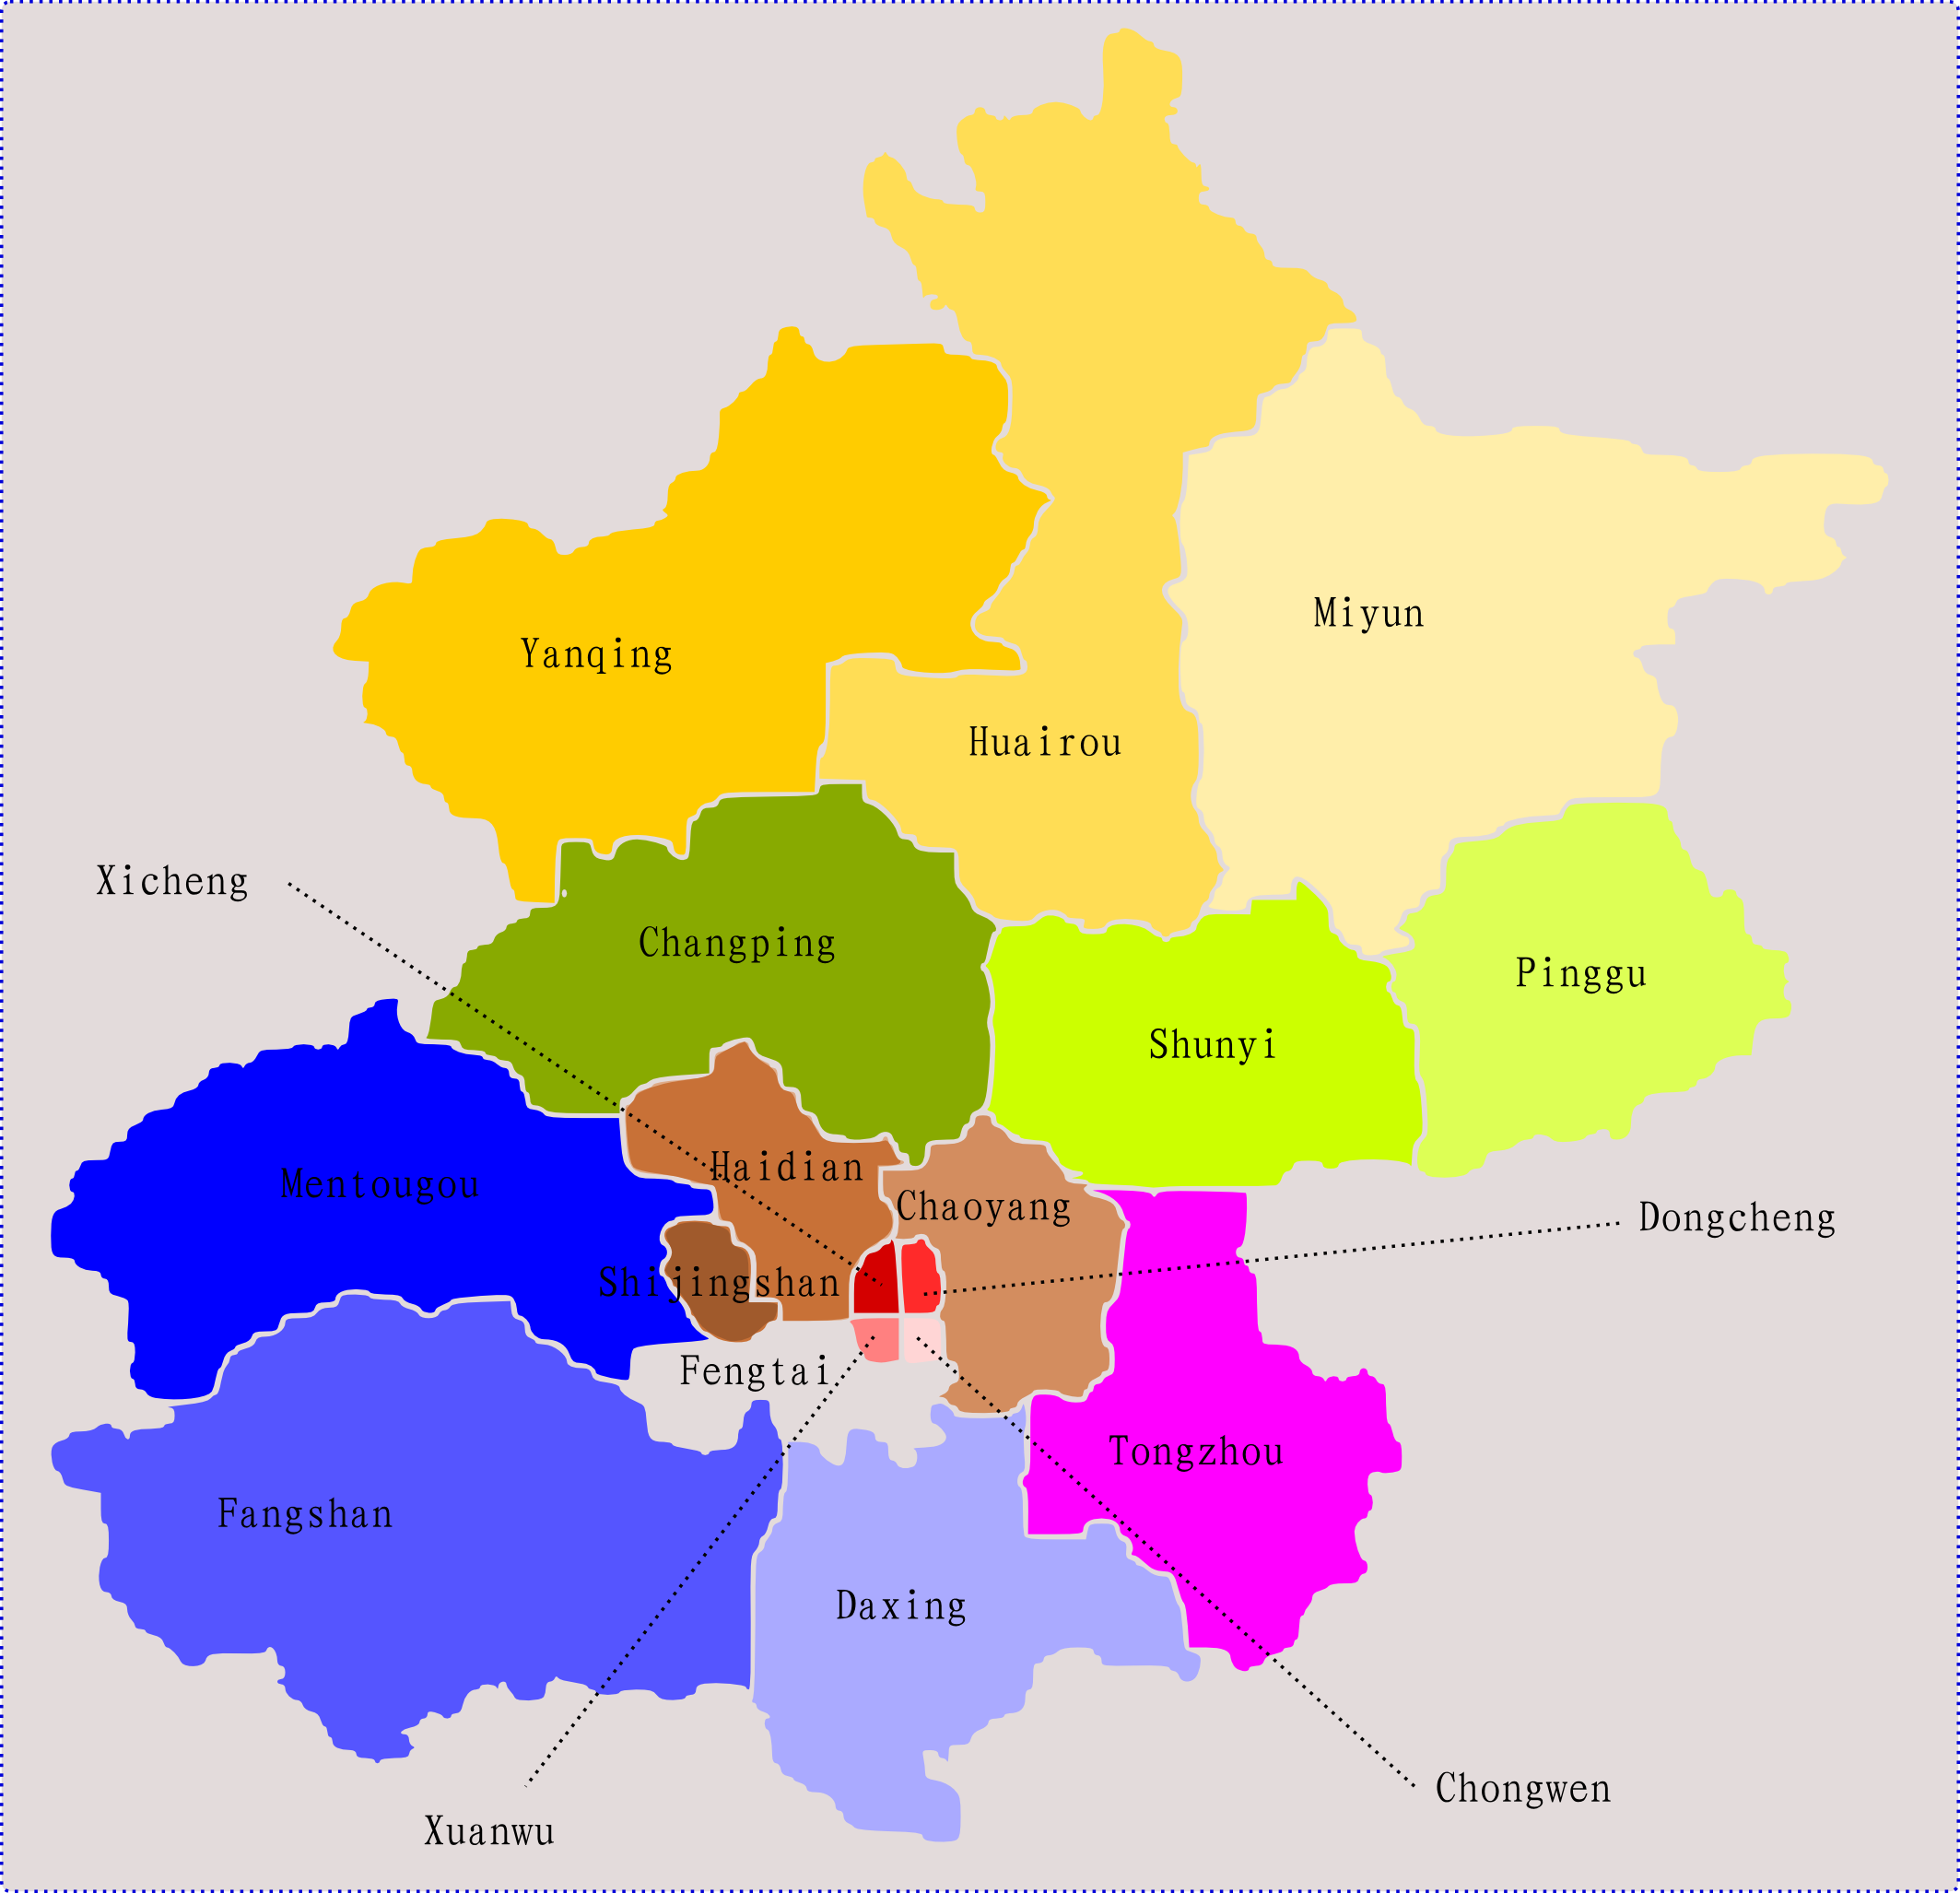
\includegraphics[width=.8\linewidth]{./images/beijing_18areas.png}
  \caption{Beijing's Districts and its Counties}
  \label{fig:data/18areas}
\end{figure}

Every day, more than X records are collected. 50, 000 records are sampled every day for a month. \selfnote{how much data can we handle} In this case, the samples correspond to April, which does not overlap with holidays and has a relatively stable weather thus diminishing the variance between bike and bus/subway traveler preferences. \domainDoubt{request a proper month data}

\subsubsection{Training data} \domainDoubt{do we have the correct classes?}
Since we perform supervised learning we need training data for which we know if a record corresponds to a commuter or non-commuter. Such data is expensive and limited since it can  only been obtained by asking the users directly if they are commuters or not. Other annotated data is not available, and labeling new records falls beyond the scope of this project. \selfnote{if data is not sufficient (although previous work shows it is) I might need to consider annotating some data myself}

The current training and validation set consists of data from 2015, collected and validated by Tu \cite{tu2016impact} \selfnote{make sure it was Tu}. The data is composed by:

\begin{itemize}
\item 6439 records of 481 commuters
\item 1628 records of 497 non-commuters
\end{itemize}

For a total of 978 IC card IDs. \selfnote{I got these from Tu, check the parameters are the same as the ones given by Liang or search for IDs in current data}

\subsubsection{Testing data}
Testing data is from 2016. More detailed

\subsection{Data preprocessing}
\subsubsection{Cleaning}
As first step for preprocessing the data, we perform a cleaning where we eliminate records that are faulty, for example: 

\begin{enumerate}
\item Eliminate records with missing data: ~10.9\% records eliminated
\item Eliminate records with travel time <= 0: <0.01\% records eliminated
\item Eliminate records with travel distance <= 0: ~10.5\% records eliminated \domainDoubt{how do we interpret these?}
\item Eliminate records linked to users with insufficient trips: ~ 25.8\% records eliminated when requiring at least 2 trips per day.
\end{enumerate}

This leaves ~52.6\% records available for usage. 

Insufficient trips regulated by a user input \selfnote{plot percentage of records and min records needed. Tune parameter}

\subsubsection{Conversion}
Parse route. Translate Chinese keywords. 

Dictionary \selfnote{encode chinese in latex}

Example in Chinese -< English -> clean route

Hourly time bins is standard practice in the field \cite{langlois2016inferring} \cite{ma2017understanding}, 

\begin{figure}[H]
  \centering
  \begin{subfigure}[b]{.45\textwidth}
  	\centering
  	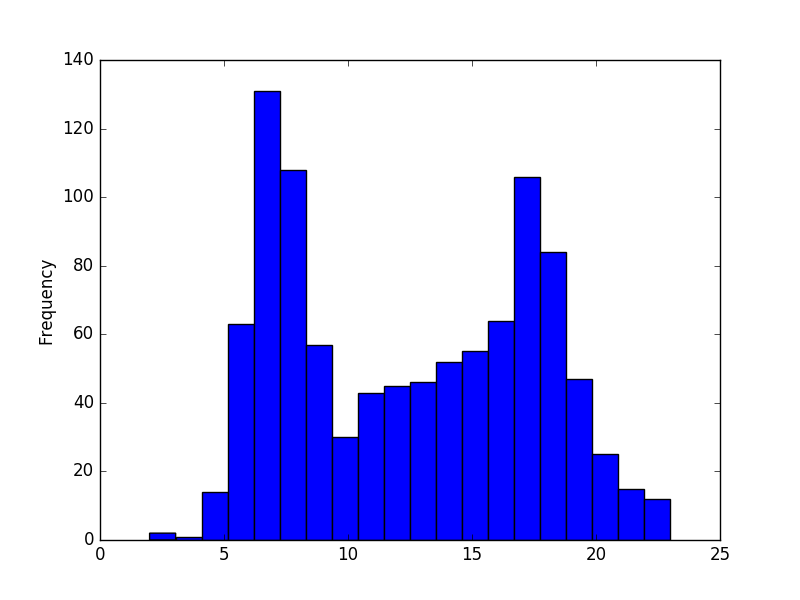
\includegraphics[width=\linewidth]{./images/start_hour_hist.png}
  	\caption{Start hour}
  \end{subfigure}
  \begin{subfigure}[b]{.45\textwidth}
  	\centering
  	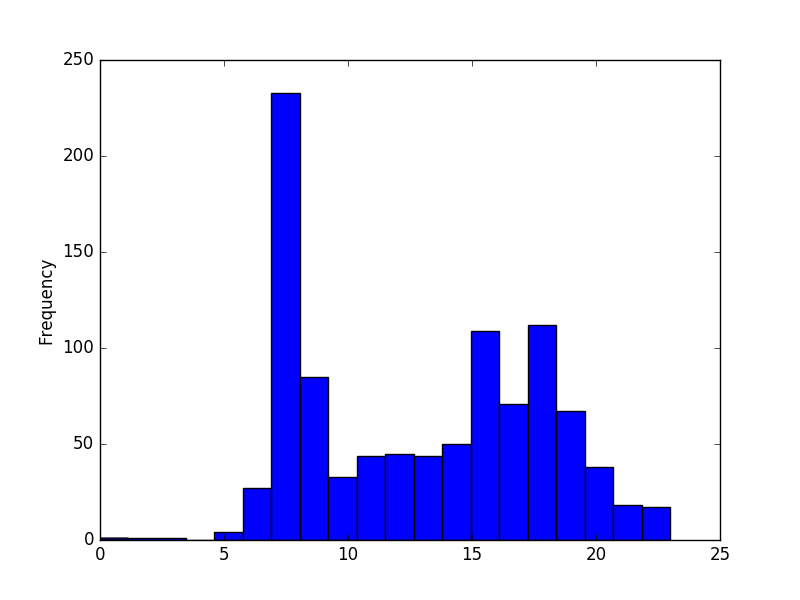
\includegraphics[width=\linewidth]{./images/end_hour_hist.png}
  	\caption{End hour}
  \end{subfigure}
  \caption{Distribution of start/end hours for trips.1000 records sample.}
  	\label{fig:preprocessing/start_end_hour}
\end{figure}

Figure \ref{fig:preprocessing/start_end_hour} shows clear morning and evening peak hours. 

\subsubsection{Standardization}
Whitening vs standardization: 

Figure \ref{fig:preprocessing/distance_time_correlation} shows a clear correlation between travel distance and travel time. \technicalDoubt{Correlation between time and distance to be preserved?}

\begin{figure}
  \centering
  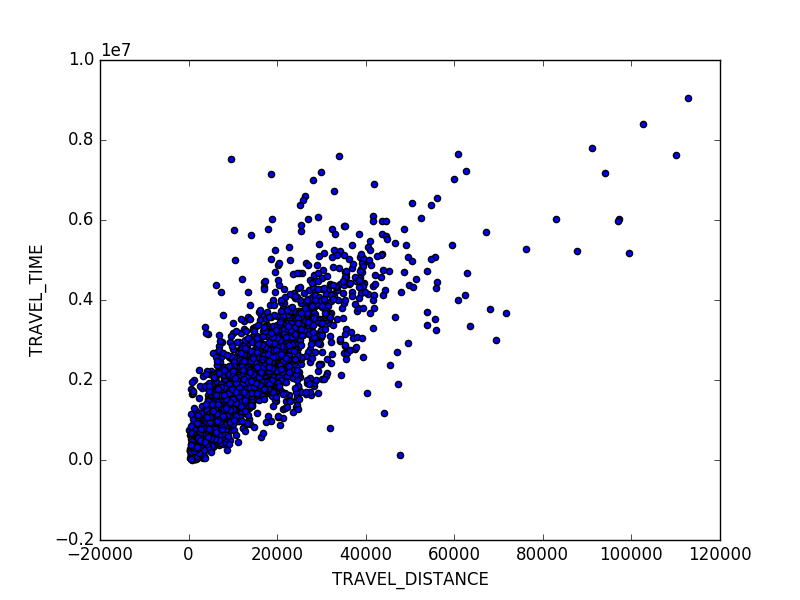
\includegraphics[width=.8\linewidth]{./images/distance_vs_time.png}
  \caption{Travel distance vs travel time.1000 record sample.}
  \label{fig:preprocessing/distance_time_correlation}
\end{figure}

Travel time and distance where standardized by subtracting the mean and forcing a standard deviation of 1 \selfnote{double check this} \selfnote{replace images once run with all data}

\begin{figure}[H]
  \centering
  \begin{subfigure}[b]{.45\textwidth}
  	\centering
  	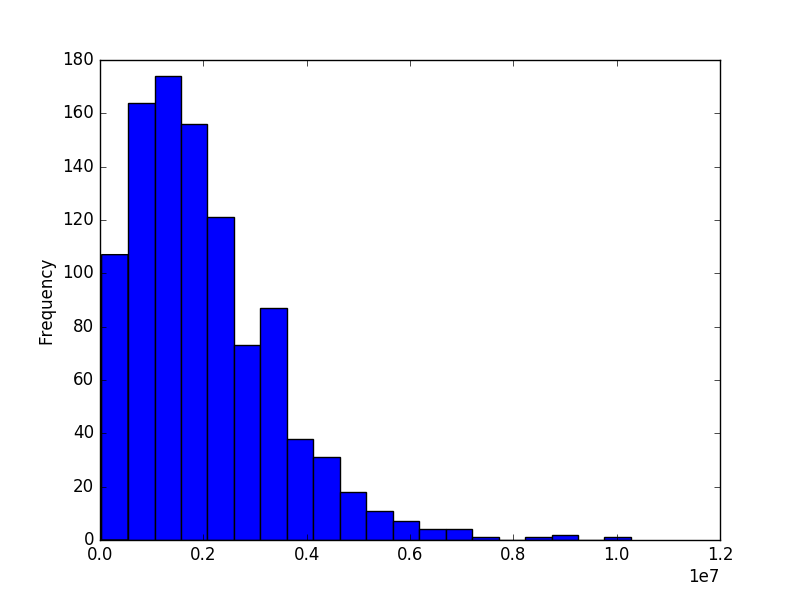
\includegraphics[width=\linewidth]{./images/time_hist.png}
  	\caption{Original}
  \end{subfigure}
  \begin{subfigure}[b]{.45\textwidth}
  	\centering
  	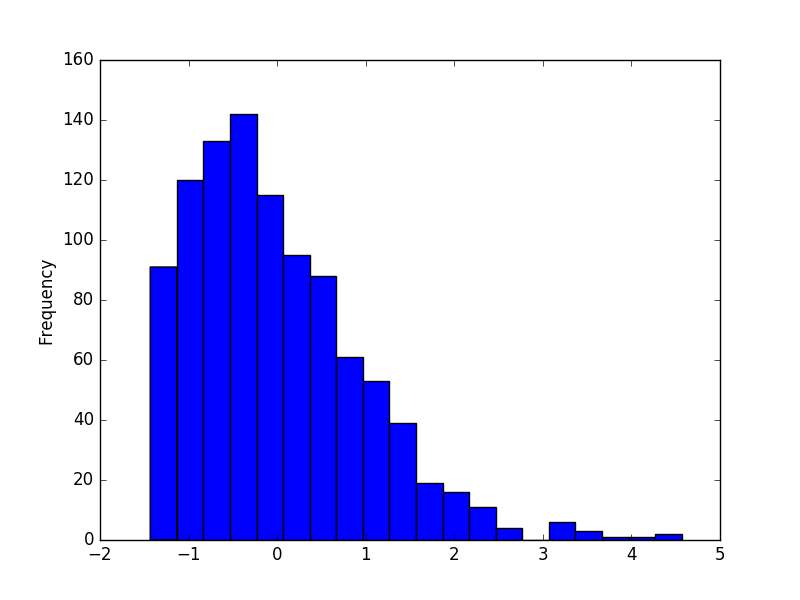
\includegraphics[width=\linewidth]{./images/time_standarized_hist.png}
  	\caption{Standarized}
  \end{subfigure}
  \caption{Time distribution before and after preprocessing. 1000 records sample.}
  	\label{fig:preprocessing/time}
\end{figure}

\begin{figure}[H]
  \centering
  \begin{subfigure}[b]{.45\textwidth}
  	\centering
  	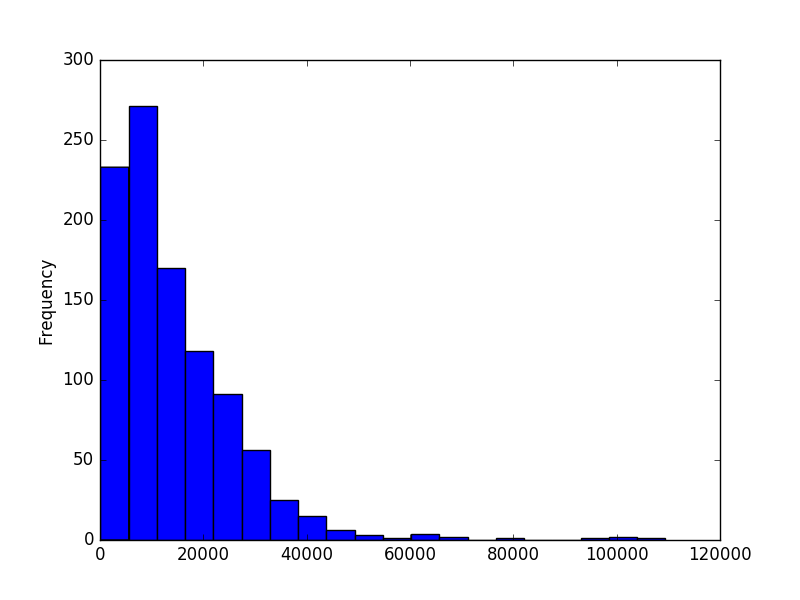
\includegraphics[width=\linewidth]{./images/distance_hist.png}
  	\caption{Original}
  \end{subfigure}
  \begin{subfigure}[b]{.45\textwidth}
  	\centering
  	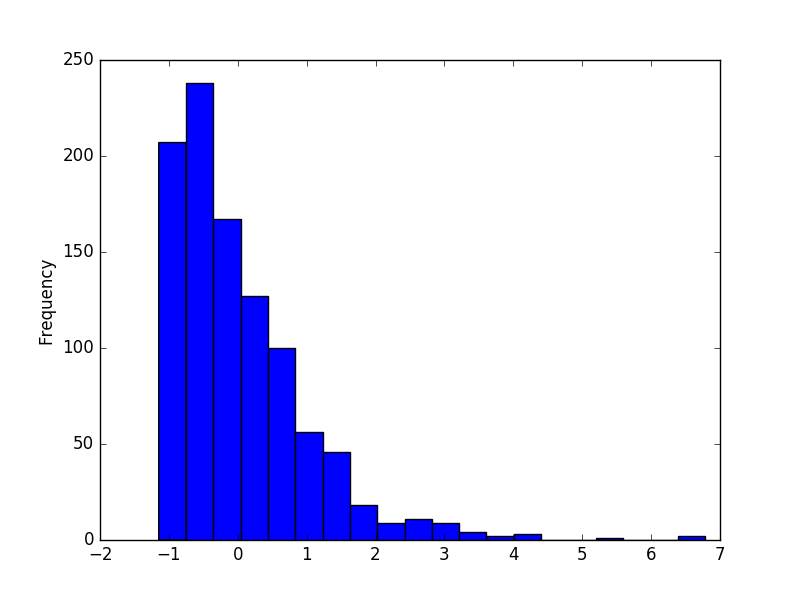
\includegraphics[width=\linewidth]{./images/distance_standarized_hist.png}
  	\caption{Standarized}
  \end{subfigure}
  \caption{Distance distribution before and after preprocessing. 1000 records sample.}
  	\label{fig:preprocessing/distance}
\end{figure}
 

\subsection{Data mining techniques}
Coding using Python. Libraries and toolboxes such as pandas, sklearn, theano.

\subsubsection{Feature engineering}
The temporal factors to be explored are represented by the start/end times, as well travel/transfer time.

The spatial factors to be explored are represented by On/Off areas. \selfnote{and route lines?}. 

\subsubsection{Ensemble models}
Ensemble models are chosen because of its robustness and modularity. Starting from two simple classifiers, assembled via bagging, the model can grow larger or more complex as needed and it may be extended beyond the scope of this Thesis Project. 

\subsubsection{Decision trees and random forests}

\subsubsection{Neural networks}

\subsection{Correlation analysis}
chi-test


\newpage
\section{Commuters identification}
\subsection{Hypothesis}
As suggested by Tu \cite{tu2016impact} results, the data is almost linearly separable thus simple classifiers such as decision trees may suffice. 


\subsection{Model}
A first instance of the model will use all available variables in the data as used by Tu \cite{tu2016impact} for a fair model comparison. 

\subsection{Experiments}

\subsection{Results}

Accuracy

Confusion matrix


\newpage
\section{Variable evaluation}
\subsection{Hypothesis}
One of the main focuses of the second phase of this thesis is to determine the appropriate level of detail in the area to be taken into account. 

Middle area, big area and (small) area overlap. Middle and small divisions have more precision but maybe not needed. On the other hand, big area divisions might not capture the changes for people who live and work/study in the same bis district. 

\subsection{Qualitative}
Exploration: Experts opinion

\subsubsection{Interview}
\selfnote{In appendix?}
We interview Liang Quan as an Transportation domain expert. 

\begin{itemize}
\item To what extent do people live and work on the same area?
\item what level of detail do you think is appropriate?
\end{itemize}

\subsection{Quantitative}
Analysis: Correlation


\newpage
\section{Commuters clustering}
\subsection{Model}

\subsection{Experiments}

\subsection{Results}

\subsection{Expert judgment}


\newpage
\section{Conclusion}


\newpage
\section{Future work}

\newpage
\bibliography{mybib}{}
\bibliographystyle{plain}

\end{document}
